\chapter{对偶空间}
\label{chap:dual-spaces}

线性映射把对象送到另一个空间。还有一类更简单的作用，只把对象读成一个数：取多项式在某一点的值，取信号的第一个样本，计算一组特征的加权和。第~\ref{sec:ls-coordinates}节的每个坐标$x_j$也是这样的读取。本章把这类线性读取本身当作研究对象，并回答三个问题：全部读取组成什么样的空间，读取怎样随线性映射在两端之间传递，以及一个读取有多大。

前两节只用线性运算。第~\ref{sec:ls-dual-space}节说明全部线性读取组成一个线性空间，即对偶空间，并用坐标读取构造它的基；第~\ref{sec:ls-dual-map}节研究对象经过线性映射以后，输出端的读取怎样传回输入端。这种传回在坐标下就是转置，它给第~\ref{chap:linear-operations}章“行列互换”的操作一个不依赖坐标的含义。

后三节加入度量结构。第~\ref{sec:ls-dual-norms}节借助第~\ref{chap:normed-spaces}章的范数度量读取的大小，即误差受限时读取的最大变化。第~\ref{sec:ls-riesz-representation}节借助第~\ref{chap:inner-product-spaces}章的内积，把每个读取写成与一个固定向量的内积；第~\ref{sec:ls-adjoints}节再把对偶映射改写成内积空间之间的映射，即伴随，并由伴随定义自伴、正交与正规算子。

本章依赖第~\ref{chap:linear-representation}章的基、坐标与线性映射，第~\ref{chap:normed-spaces}章的范数与诱导矩阵范数，以及第~\ref{chap:inner-product-spaces}章的内积、Gram矩阵与标准正交基。全章只讨论有限维空间；无限维空间中并非每个线性泛函都连续，那里的对偶理论属于函数空间。

% 对偶空间：线性泛函、对偶空间与对偶基。

\section{线性泛函}
\label{sec:ls-dual-space}
\phantomsection
\label{sec:ls-dual-spaces}

\paragraph{线性泛函的定义}
保持线性组合的标量读取称为\term{线性泛函}（linear functional），即满足
\[
\varphi(a\bm x+b\bm y)=a\varphi(\bm x)+b\varphi(\bm y),\qquad\bm x,\bm y\in V,\ a,b\in\mathbb R
\]
的映射$\varphi:V\to\mathbb R$。它就是陪域为$\mathbb R$的线性映射。在$P_k$上，取值$p\mapsto p(t_0)$与积分$p\mapsto\int_0^1p(t)\,\mathrm dt$都是线性泛函；在$\mathbb R^d$上，读取第$j$个坐标与加权和$\bm x\mapsto\bm a^\top\bm x$都是线性泛函。但并非每个把向量读成一个数的规则都是线性泛函。
\begin{example}[反例：两个非线性的读取]
\label{ex:ls-nonlinear-readouts}
考虑$\mathbb R^d$上的两个读取：$\varphi_1(\bm x)=x_1+1$把第一个坐标加上$1$，$\varphi_2(\bm x)=\lVert\bm x\rVert_2$读出长度。线性泛函必把零向量读成$0$，而$\varphi_1(\bm0)=1$，常数项已经破坏了线性。$\varphi_2$在零向量处读数为$0$，问题出在符号上：线性泛函满足$\varphi(-\bm x)=-\varphi(\bm x)$，但对任一$\bm x\neq\bm0$，$\varphi_2(-\bm x)=\lVert\bm x\rVert_2>0$，而$-\varphi_2(\bm x)<0$。所以二者都不是线性泛函。
\end{example}

线性泛函是线性映射，所以也有矩阵表示。选定$V$的基$\mathcal B=(\bm b_1,\ldots,\bm b_d)$，输出端取数$1$作基，线性泛函$\varphi$记录为$1\times d$矩阵：
\[
 \begin{gathered}
[\varphi]_{\mathcal B}=\bigl(\varphi(\bm b_1),\ \ldots,\ \varphi(\bm b_d)\bigr)\\
\varphi(\bm v)=[\varphi]_{\mathcal B}[\bm v]_{\mathcal B}=\sum_{j=1}^dx_j\varphi(\bm b_j).
 \end{gathered}
\]
对象的坐标是一列，读取规则的系数是一行，二者相乘得到读数。

非零泛函的核与像也容易确定。非零泛函取到某个非零值，把相应的输入缩放即可取到任意实数，所以它的像是整个$\mathbb R$；由秩零度定理，它的核是$d-1$维子空间。读数等于$c$的点组成核的平移$\bm x_0+\ker\varphi$（其中$\varphi(\bm x_0)=c$），在平面上就是一族平行直线。

\paragraph{对偶空间}
同一个对象可以接受多种读取，两种读取也可以组合。规定
\[
 (\alpha\varphi+\beta\psi)(\bm x)=\alpha\varphi(\bm x)+\beta\psi(\bm x),
\]
右端对$\bm x$仍保持线性组合，所以线性泛函的线性组合仍是线性泛函。全部线性泛函在这两种运算下构成线性空间，称为$V$的\term{对偶空间}（dual space），记为$V^*$。输入向量是被读取的对象，泛函是读取规则，二者属于不同的空间。即使在$\mathbb R^d$中一行系数与一列坐标的数字相同，也不能把二者相加。

\paragraph{对偶基}
坐标给出了一组现成的读取，用它们可以确定$V^*$的维数。对$V$的有序基$\mathcal B=(\bm b_1,\ldots,\bm b_d)$，第$j$个坐标$\bm v\mapsto x_j$是线性泛函（坐标映射保持线性组合），记为$\varphi_j$。由于$\bm b_i$的坐标是$\bm e_i$，
\begin{equation}
 \varphi_j(\bm b_i)=\delta_{j,i}
 =\begin{cases}1,&i=j,\\0,&i\neq j.\end{cases}
 \label{eq:ls-dual-basis-def}
\end{equation}
反过来，线性泛函由它在基向量上的值决定，所以式~\eqref{eq:ls-dual-basis-def}也可以当作$\varphi_j$的定义。

这$d$个读取构成$V^*$的一组基。它们张成$V^*$：任意$\varphi\in V^*$都能写成
\[
 \varphi=\sum_{j=1}^d\varphi(\bm b_j)\,\varphi_j,
\]
因为两边在每个$\bm b_i$上取值都是$\varphi(\bm b_i)$，而线性泛函由基向量上的值决定。它们线性无关：若$\sum_ja_j\varphi_j=0$，在$\bm b_i$上取值得$a_i=0$。

$\varphi_1,\ldots,\varphi_d$称为$\mathcal B$的\term{对偶基}（dual basis），于是$\dim V^*=\dim V$。读取$\varphi$在对偶基下的坐标，正是它在各基向量上的读数$\varphi(\bm b_j)$，也就是上面那一行系数。

对偶基的每个成员依赖整组基，而不只依赖对应的那个基向量。
\begin{example}[改变第二个基向量会改变第一个坐标读取]
\label{ex:ls-dual-basis-depends-on-basis}
比较$\mathbb R^2$的标准基$(\bm e_1,\bm e_2)$与基$(\bm e_1,\bm e_1+\bm e_2)$，两者只有第二个向量不同。标准基的对偶基是两个坐标读取$\varphi_1(x,y)=x$、$\varphi_2(x,y)=y$。在第二组基下，把$(x,y)^\top$重新分解为
\[
 (x,y)^\top=(x-y)\bm e_1+y(\bm e_1+\bm e_2),
\]
所以第一个坐标读取变成$x-y$，第二个坐标读取仍是$y$。第一个基向量始终是$\bm e_1$，相应的对偶读取却从$x$变成了$x-y$。原因是新的第二个基向量也含有$\bm e_1$分量，第一个读取必须扣除由它贡献的那部分。
\end{example}
对一般的基，对偶基要由方程组$\varphi_j(\bm b_i)=\delta_{j,i}$解出。
\begin{example}[斜基的对偶基]
\label{ex:ls-dual-basis-oblique}
取$\mathbb R^2$的基$\bm b_1=(2,1)^\top$、$\bm b_2=(-1,1)^\top$，先求它的对偶基。线性泛函都形如$\varphi_1(x,y)=\alpha x+\beta y$，所以只需定出两个系数。条件$\varphi_1(\bm b_1)=2\alpha+\beta=1$与$\varphi_1(\bm b_2)=-\alpha+\beta=0$给出$\alpha=\beta=1/3$；同样由$\varphi_2(\bm b_1)=0$、$\varphi_2(\bm b_2)=1$解出$\varphi_2$，得
\[
 \begin{gathered}
\varphi_1(x,y)=\frac{x+y}3\\
\varphi_2(x,y)=\frac{-x+2y}3 .
 \end{gathered}
\]
再用这组对偶基表示读取横坐标的泛函$\ell(x,y)=x$。按前面的展开式，系数就是$\ell$在基向量上的读数$\ell(\bm b_1)=2$、$\ell(\bm b_2)=-1$，所以$\ell=2\varphi_1-\varphi_2$。代入验证：$\tfrac23(x+y)-\tfrac13(-x+2y)=x$。可见求读取在对偶基下的坐标不必解方程，只要把它作用在各基向量上。
\end{example}
图~\ref{fig:ls-dual-basis-readout}画出这些读取：每个对偶读取只在一个基向量上读到$1$，在另一个基向量上读到$0$。
\begin{figure}[htbp]
  \centering
  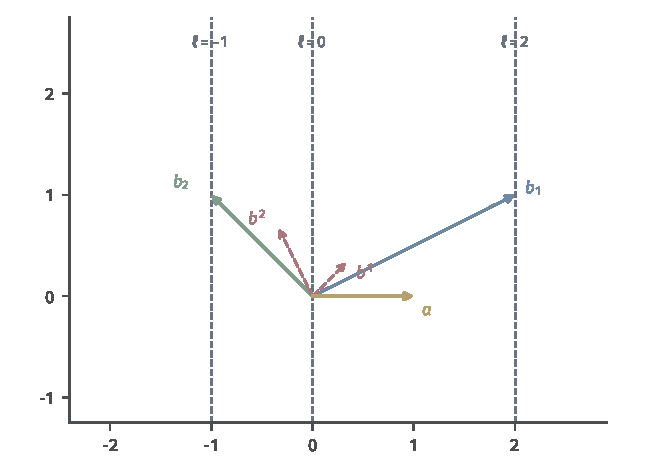
\includegraphics[width=112mm]{figures/00-shared/mathematical-preliminaries-upper/02-linear-spaces/matplotlib/ls-dual-basis-readout/ls-dual-basis-readout.pdf}
  \caption{对偶读取的几何示意。蓝箭头$\bm b_1=(2,1)$、绿箭头$\bm b_2=(-1,1)$为基向量；红色虚线箭头$\bm b^1=(1/3,1/3)$、$\bm b^2=(-1/3,2/3)$分别是对偶基$\varphi_1,\varphi_2$的系数向量，即$\varphi_i(\bm x)=\bm b^i\cdot\bm x$，满足$\varphi_i(\bm b_j)=\delta_{i,j}$。把读取规则画成平面箭头借用了标准内积，这一对应在第~\ref{sec:ls-riesz-representation}节说明。黄色箭头$\bm a=(1,0)$给出读取$\ell(\bm x)=\bm a\cdot\bm x$，灰色虚线为等值线$\ell=c$（$c=-1,0,2$）；$\ell(\bm b_1)=2$、$\ell(\bm b_2)=-1$，且$\bm a=2\bm b^1-\bm b^2$。}
  \label{fig:ls-dual-basis-readout}
\end{figure}

换基时，读取系数与坐标按相反的方向变化。设新基$\mathcal B'$由换基矩阵$\bm P=\bm S_{\mathcal B\leftarrow\mathcal B'}$给出，即$\bm b'_j=\sum_i\bm P_{i,j}\bm b_i$。坐标按
\[
 [\bm v]_{\mathcal B'}=\bm P^{-1}[\bm v]_{\mathcal B}
\]
变化；读取系数则按$\varphi(\bm b'_j)=\sum_i\varphi(\bm b_i)\bm P_{i,j}$变化，即
\[
 [\varphi]_{\mathcal B'}=[\varphi]_{\mathcal B}\bm P.
\]
二者相乘时$\bm P$与$\bm P^{-1}$相消，所以读数$\varphi(\bm v)$不随基改变，这正是读数应有的性质。

% 对偶空间：对偶映射与转置。

\section{对偶映射}
\label{sec:ls-dual-map}

已知线性映射$T:V\to W$和输出端的一个读取$f\in W^*$，输入$\bm x$经过$T$以后被读成$f(T\bm x)$。先作用、再读取，合起来是输入端的一个读取。由这一复合定义\term{对偶映射}（dual map）$T':W^*\to V^*$：
\begin{equation}
\begin{gathered}
T'f=f\circ T\\
(T'f)(\bm x)=f(T\bm x).
\end{gathered}
\label{eq:ls-dual-map-def}
\end{equation}
$T'$保持线性组合：$(T'(\alpha f+\beta g))(\bm x)=\alpha f(T\bm x)+\beta g(T\bm x)$。对象从$V$走到$W$，读取则从$W^*$传回$V^*$，方向相反；这只是把读取规则搬回输入端，不是对$T$求逆。

复合时次序也随之反转：对$S:W\to U$，$(S\circ T)'f=f\circ S\circ T=T'(S'f)$，即$(S\circ T)'=T'\circ S'$。

\paragraph{对偶映射的矩阵是转置}
设$T$在输入基$\mathcal B=(\bm b_1,\ldots,\bm b_d)$、输出基$\mathcal C=(\bm c_1,\ldots,\bm c_m)$下的矩阵为$\bm A$，即$T\bm b_j=\sum_ka_{k,j}\bm c_k$；两组基的对偶基分别记为$\varphi_1,\ldots,\varphi_d$与$\psi_1,\ldots,\psi_m$。取输出读取$f=\sum_iy_i\psi_i$，它传回输入端以后，在输入基向量上的读数是
\[
 (T'f)(\bm b_j)=f(T\bm b_j)
 =\sum_iy_i\,\psi_i\Bigl(\sum_ka_{k,j}\bm c_k\Bigr)
 =\sum_ia_{i,j}y_i=(\bm A^\top\bm y)_j .
\]
上一节说明，读取在对偶基下的坐标就是它在各基向量上的读数，所以$T'f$的坐标为$\bm A^\top\bm y$。也就是说，在对偶基下，对偶映射的矩阵是$\bm A^\top$。转置的乘积规则$(\bm B\bm A)^\top=\bm A^\top\bm B^\top$正是$(S\circ T)'=T'\circ S'$的坐标记录。下面用一个具体映射核对这一结论。
\begin{example}[把输出的第一个分量读取传回输入端]
\label{ex:ls-dual-map-first-component}
再看$T(x_1,x_2)=(2x_1+x_2,\ 3x_2)$，它在标准基下的矩阵为
\[
 \bm A=\begin{bmatrix}2&1\\0&3\end{bmatrix}.
\]
在输出端读取第一个分量，即$f=\psi_1$，系数$\bm y=(1,0)^\top$。按定义先作用再读取，$(T'f)(\bm x)=f(T\bm x)=2x_1+x_2$，传回输入端的读取系数为$(2,1)^\top$。按转置计算，$\bm A^\top(1,0)^\top=(2,1)^\top$，两种算法一致。这组系数正是$\bm A$的第一行：输出的第一个分量本来就由第一行与输入相乘得到。
\end{example}
一般地，读取输出的第$i$个分量并传回输入端，得到的读取系数就是$\bm A$的第$i$行，所以$T'$的像在坐标下就是行空间。

\paragraph{再证行秩等于列秩}
对偶映射给出定理~\ref{thm:ls-row-rank-column-rank}的另一个证明，它不把矩阵分解为两个因子，而是计算$T'$的核。$T'f=0$意味着$f(T\bm x)=0$对一切$\bm x$成立，即$f$在$\operatorname{im}T$上恒为零。所以$\ker T'$由对全部可达输出读数为零的读取组成，在坐标下就是$\bm A^\top\bm y=\bm0$，即左零空间。

下面计算它的维数。设$r=\operatorname{rank}T$，取$\operatorname{im}T$的基$\bm c_1,\ldots,\bm c_r$并扩充为$W$的基$\bm c_1,\ldots,\bm c_m$，对偶基为$\psi_1,\ldots,\psi_m$。读取$f=\sum_iy_i\psi_i$在$\operatorname{im}T$上恒为零，当且仅当它在$\bm c_1,\ldots,\bm c_r$上都读到零，即$y_1=\cdots=y_r=0$。所以$\ker T'=\operatorname{span}\{\psi_{r+1},\ldots,\psi_m\}$，维数为$m-r$。

对$T':W^*\to V^*$用秩零度定理，$\operatorname{rank}T'=\dim W^*-\dim\ker T'=m-(m-r)=r$。$T'$的矩阵是$\bm A^\top$，于是$\operatorname{rank}\bm A^\top=\operatorname{rank}\bm A$。

读取规则至此有了自己的空间、坐标和传递规律。读取的大小，即输入有界时读数最大能有多大，需要先给输入规定范数，由第~\ref{sec:ls-dual-norms}节的对偶范数回答；读取能否写成与某个固定向量的内积，由第~\ref{sec:ls-riesz-representation}节回答。

% 对偶空间：对偶范数。

\section{对偶范数}
\label{sec:ls-dual-norms}

第~\ref{sec:ls-dual-spaces}节的线性泛函是对向量的读取。有了范数，就可以衡量一个读取有多大。误差分析中的典型问题是：误差$\bm r$只知道落在某个范数球内，一次加权读取$\bm z^\top\bm r$最多变化多少。在$\mathbb R^d$上取定一种范数后，这个最大值就是对偶范数。
\begin{definition}[对偶范数]
\label{def:linear-algebra-dual-norm}
给定$\mathbb R^d$上的范数，相对于标准坐标配对的\term{对偶范数}（dual norm）为
\begin{equation}
 \lVert\bm z\rVert_*=\sup_{\lVert\bm r\rVert\leq1}|\bm z^\top\bm r|.
 \label{eq:linear-algebra-dual-norm-definition}
\end{equation}
\end{definition}
这就是第~\ref{sec:ls-matrix-norms}节的诱导范数取输出空间为$\mathbb R$的情形：读取$\bm r\mapsto\bm z^\top\bm r$是$1\times d$矩阵$\bm z^\top$的作用。所以对任意范数，上确界有限并且可以取到。

对偶范数满足范数的各条要求，因而是对偶空间上的范数。非负性显然。$\bm z\neq\bm0$时，取$\bm z$的某个非零坐标$z_j$，则$\bm r=\bm e_j/\lVert\bm e_j\rVert$给出$|\bm z^\top\bm r|=|z_j|/\lVert\bm e_j\rVert>0$，这给出正定性。对每个$\bm r$都有$|(\bm z+\bm w)^\top\bm r|\leq|\bm z^\top\bm r|+|\bm w^\top\bm r|$，取上确界即得三角不等式；齐次性由$|(c\bm z)^\top\bm r|=|c|\,|\bm z^\top\bm r|$得到。图~\ref{fig:ls-dual-norm-unit-ball}把这个最大值画成支撑线最后接触单位球的位置。

\begin{figure}[!htb]
  \centering
  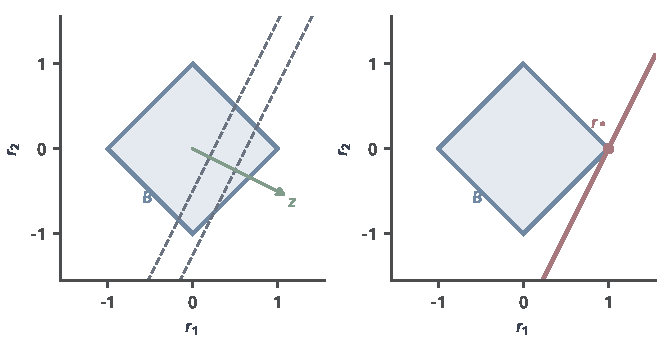
\includegraphics[width=112mm]{figures/00-shared/mathematical-preliminaries-upper/02-linear-spaces/matplotlib/ls-dual-norm-unit-ball/ls-dual-norm-unit-ball.pdf}
  \caption{对偶范数的几何：在原范数单位球$\lVert\bm r\rVert\leq1$上求线性读取$\bm z^\top\bm r$的最大值。左：原单位球（灰色）与读取方向$\bm z$；右：支撑直线最后接触单位球处给出$\lVert\bm z\rVert_*=\max_{\lVert\bm r\rVert\leq1}|\bm z^\top\bm r|$。对偶单位球（虚线）与原单位球互为极体。解析教学例。}
  \label{fig:ls-dual-norm-unit-ball}
\end{figure}

对$\ell_p$范数，对偶范数可以明确写出：
\begin{equation}
(\lVert\cdot\rVert_p)_*=\lVert\cdot\rVert_q,\qquad\frac1p+\frac1q=1.
\label{eq:linear-algebra-lp-duality}
\end{equation}
由齐次性，对任意预算$\rho\geq0$还有
\begin{equation}
 \max_{\lVert\bm r\rVert_p\leq\rho}|\bm z^\top\bm r|
 =\rho\lVert\bm z\rVert_q.
 \label{eq:linear-algebra-linear-perturbation-duality}
\end{equation}
Hölder不等式（定理~\ref{thm:linear-algebra-holder}）给出$\ell_p$单位球上的上界$\lVert\bm z\rVert_q$。这个上界可以达到。$1<p<\infty$且$\bm z\neq\bm0$时，取$r_j=|z_j|^{q-1}\operatorname{sgn}(z_j)/\lVert\bm z\rVert_q^{q-1}$；$\bm z=\bm0$时上界为零，任取可行输入即可。$p=1$时，把单位预算全部放在$|z_j|$最大的坐标上；$p=\infty$时，逐坐标取$r_j=\operatorname{sgn}(z_j)$。下面固定一个读取，比较三种误差预算。
\begin{example}[同一读取在三种误差预算下的最大变化]
\label{ex:ls-dual-norm-three-budgets}
取读取方向$\bm z=(2,-1)^\top$，即读取$\bm z^\top\bm r=2r_1-r_2$，让误差$\bm r$分别落在三种单位球内。

在$\ell_1$单位球上，预算只能分给各坐标的绝对值，全部放在权重$|z_j|$最大的第一个坐标最划算：$\bm r=(1,0)^\top$给出最大值$\lVert\bm z\rVert_\infty=2$。在$\ell_2$单位球上，最坏误差与$\bm z$同方向，取$\bm r=\bm z/\lVert\bm z\rVert_2=(2,-1)^\top/\sqrt5$，最大值为$\lVert\bm z\rVert_2=\sqrt5$。在$\ell_\infty$单位球上，每个坐标都可以同时取满，只需让符号与$z_j$一致：$\bm r=(1,-1)^\top$给出最大值$\lVert\bm z\rVert_1=3$。换成实际的误差预算$|r_j|\leq0.01$，就在式~\eqref{eq:linear-algebra-linear-perturbation-duality}中取$p=\infty$、$\rho=0.01$，最大变化为$0.01\cdot(2+1)=0.03$，由$\bm r=(0.01,-0.01)^\top$达到。

三种单位球给出的最大值依次为$2$、$\sqrt5$、$3$。读取本身没有变，变的是允许误差的形状：它决定了最坏方向在哪里，也决定了读取方向要用哪个对偶范数计量。
\end{example}
图~\ref{fig:linear-algebra-dual-unit-balls}画出这三种情形下的最坏方向。
\begin{figure*}[htbp]
  \centering
  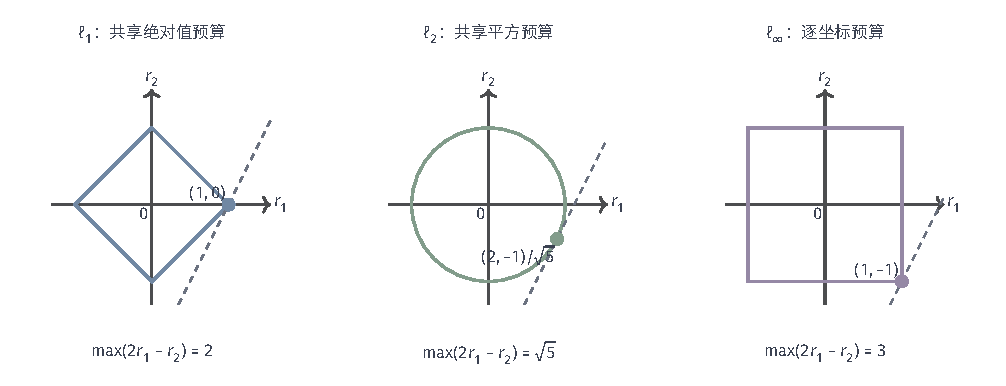
\includegraphics[width=168.998mm]{figures/00-shared/mathematical-preliminaries-upper/02-linear-spaces/tikz/linear-algebra-dual-unit-balls/figure.pdf}
  \caption{同一线性读取$2r_1-r_2$在$\ell_1$、$\ell_2$、$\ell_\infty$单位球上的最大值依次为$2$、$\sqrt5$、$3$。虚线为最后接触可行集的支撑直线，点为最大化方向。三图坐标尺度相同，均为解析教学例；允许误差的形状改变时，误差常数也随之改变。}
  \label{fig:linear-algebra-dual-unit-balls}
\end{figure*}

由此可见，误差预算按$\ell_\infty$给出时，读取方向要按$\ell_1$计量；预算按$\ell_2$给出时，读取方向仍按$\ell_2$计量。

原空间的范数改变，对偶范数随之改变。对加权的坐标范数，可以用换元把问题化回已知情形。
\begin{example}[加权$\ell_1$范数的对偶范数]
\label{ex:ls-weighted-dual-norm}
设权重$w_1,\ldots,w_d>0$，在$\mathbb R^d$上取加权范数$\lVert\bm r\rVert_{\bm w}=\sum_jw_j|r_j|$。把权重吸收进变量，令$s_j=w_jr_j$，则$\lVert\bm r\rVert_{\bm w}=\lVert\bm s\rVert_1$，$\bm z^\top\bm r=\sum_j(z_j/w_j)s_j$。$\bm r$取遍$\lVert\bm r\rVert_{\bm w}\leq1$时，$\bm s$恰好取遍$\ell_1$单位球。由式~\eqref{eq:linear-algebra-lp-duality}中$p=1$的情形，
\[
 \lVert\bm z\rVert_*=\max_j\frac{|z_j|}{w_j}.
\]
仍取上例的$\bm z=(2,-1)^\top$。不加权，即$\bm w=(1,1)^\top$时，$\lVert\bm z\rVert_*=2$，由$\bm r=(1,0)^\top$取到，与上例的$\ell_1$情形一致；改用$\bm w=(4,1)^\top$时，$\lVert\bm z\rVert_*=\max\{1/2,1\}=1$，由$\bm r=(0,-1)^\top$取到。

读取$\bm z^\top\bm r$的代数表达没有变，它的大小却随原空间的范数改变。第一个坐标的权重变大后，同样的预算只允许它有更小的变化，最坏方向因而转到第二个坐标。
\end{example}
所以讨论“输入误差最多引起多大输出误差”时，必须先说清误差用哪种范数度量。内积诱导的范数下，对偶范数等于表示向量的长度，在第~\ref{sec:ls-riesz-representation}节证明。一般有限维空间$V$上的线性泛函$\varphi$同样定义$\lVert\varphi\rVert_*=\max_{\lVert\bm v\rVert\leq1}|\varphi(\bm v)|$，它是取$W=\mathbb R$时的算子范数。无限维空间中，并非每个线性泛函都连续，代数对偶与连续对偶需要区分，这同样属于无限维理论。

% 对偶空间：线性泛函的内积表示。

\section{线性泛函的内积表示}
\phantomsection
\label{sec:ls-riesz-representation}
在$\mathbb R^d$的欧氏内积下，加权读取$\varphi(\bm x)=\bm a^\top\bm x$就是与向量$\bm a$的内积。在一般有限维内积空间中，每个读取也都能这样写。
\begin{theorem}[有限维Riesz表示定理]
\label{thm:ls-riesz-representation}
设$V$是有限维内积空间。对每个$\varphi\in V^*$，存在唯一的$\bm v_\varphi\in V$，使$\varphi(\bm x)=\langle\bm x,\bm v_\varphi\rangle$对所有$\bm x\in V$成立。
\end{theorem}
\begin{proof}
取$V$的一组标准正交基$\bm q_1,\ldots,\bm q_d$（第~\ref{sec:ls-orthonormal-basis-construction}节），令$\bm v_\varphi=\sum_j\varphi(\bm q_j)\bm q_j$。由式~\eqref{eq:ls-orthonormal-expansion}，$\bm x=\sum_j\langle\bm x,\bm q_j\rangle\bm q_j$，于是
\[
 \varphi(\bm x)=\sum_j\langle\bm x,\bm q_j\rangle\varphi(\bm q_j)=\Bigl\langle\bm x,\sum_j\varphi(\bm q_j)\bm q_j\Bigr\rangle=\langle\bm x,\bm v_\varphi\rangle.
\]
若$\bm v,\bm v'$都满足要求，则$\langle\bm x,\bm v-\bm v'\rangle=0$对一切$\bm x$成立，取$\bm x=\bm v-\bm v'$得$\bm v=\bm v'$。
\end{proof}
对应$\varphi\mapsto\bm v_\varphi$保持线性组合，这由表示向量的唯一性得到；每个$\bm v$又都表示读取$\langle\cdot,\bm v\rangle$。所以这个对应是$V^*$到$V$的双射。在它之下，标准正交基的对偶基就是这组基本身，因为第$j$个坐标读取是$\bm x\mapsto\langle\bm x,\bm q_j\rangle$。对一般的基，对偶基对应的向量与原基不同：图~\ref{fig:ls-dual-basis-readout}中的红色箭头$\bm b^1,\bm b^2$，正是对偶读取$\varphi_1,\varphi_2$在欧氏内积下对应的向量。

表示向量依赖内积，读取本身却不依赖。在$\mathbb R^d$上取加权内积$\langle\bm x,\bm y\rangle_{\bm M}=\bm x^\top\bm M\bm y$，同一个读取$\varphi(\bm x)=\bm a^\top\bm x=\bm x^\top\bm M(\bm M^{-1}\bm a)$对应的向量是$\bm M^{-1}\bm a$，而不是$\bm a$。函数空间中也是如此。
\begin{example}[积分读取在两点内积下的表示向量]
\label{ex:ls-riesz-integral-two-point}
在$P_1$上取两点内积$\langle f,g\rangle=f(0)g(0)+f(1)g(1)$，考虑积分读取$\varphi(f)=\int_0^1f(t)\,\mathrm dt$。对$f=a+bt$，$\varphi(f)=a+b/2$。要把它写成与某个固定函数的内积，而这个内积只用到$f(0)=a$与$f(1)=a+b$，所以先把$a+b/2$表示成这两个值的组合：$a+b/2=\tfrac12\bigl(f(0)+f(1)\bigr)$。这正是$f$与常数函数$\tfrac12$的内积：
\[
 \Bigl\langle f,\tfrac12\Bigr\rangle=\tfrac12\bigl(f(0)+f(1)\bigr)=\tfrac12(a+a+b)=a+\frac b2 .
\]

因此$\bm v_\varphi$是常数函数$\tfrac12$。在系数向量的欧氏内积下，同一个读取对应$(1,1/2)^\top$，表示向量随内积而变。等式$\varphi(f)=\tfrac12\bigl(f(0)+f(1)\bigr)$也说明梯形公式对一次函数精确。
\end{example}
表示向量还给出读取的大小。由Cauchy--Schwarz不等式，$|\varphi(\bm x)|\leq\lVert\bm x\rVert\,\lVert\bm v_\varphi\rVert$；$\bm v_\varphi\neq\bm0$时，取$\bm x=\bm v_\varphi/\lVert\bm v_\varphi\rVert$可取到等号。所以仿照第~\ref{sec:ls-dual-norms}节，在单位球上取读取的最大值，得到
\[
 \lVert\varphi\rVert_*=\max_{\lVert\bm x\rVert\leq1}|\varphi(\bm x)|=\lVert\bm v_\varphi\rVert .
\]
在$\mathbb R^d$的欧氏内积下，这就是$\ell_2$范数的对偶范数仍为$\ell_2$范数。

% 对偶空间：伴随与特殊线性算子。

\section{伴随与特殊线性算子}
\label{sec:ls-adjoints}
对偶映射把输出端的读取$f$传回输入端，得到读取$f\circ T$。若把两端的读取都换成表示它的向量，就得到伴随。
\begin{definition}[伴随]
\label{def:linear-algebra-adjoint}
设$T:V\to W$是两个有限维实内积空间之间的线性映射。若存在$T^\star:W\to V$使
\begin{equation}
 \langle T\bm x,\bm y\rangle_W=\langle\bm x,T^\star\bm y\rangle_V
 \label{eq:ls-adjoint-pairing}
\end{equation}
对所有$\bm x\in V$、$\bm y\in W$成立，则$T^\star$称为$T$的\term{伴随}（adjoint）。
\end{definition}

伴随总存在且唯一。固定$\bm y\in W$，$\bm x\mapsto\langle T\bm x,\bm y\rangle_W$是$V$上的线性泛函。由定理~\ref{thm:ls-riesz-representation}，存在唯一的向量使它写成与该向量的内积，把这个向量记为$T^\star\bm y$。$T^\star$对$\bm y$线性：
\[
 \langle\bm x,aT^\star\bm y+bT^\star\bm y'\rangle_V=a\langle T\bm x,\bm y\rangle_W+b\langle T\bm x,\bm y'\rangle_W=\langle T\bm x,a\bm y+b\bm y'\rangle_W,
\]
由表示向量的唯一性，$T^\star(a\bm y+b\bm y')=aT^\star\bm y+bT^\star\bm y'$。

用对偶映射的语言说，把$\bm y\in W$看成读取$\langle\cdot,\bm y\rangle_W$，则$T'$把它送到读取$\langle T\,\cdot,\bm y\rangle_W=\langle\cdot,T^\star\bm y\rangle_V$。所以伴随就是借内积把读取换成向量以后的对偶映射。

具体计算时，取$V,W$的基。由坐标下的内积公式，两边的内积写成$\langle\bm x,\bm x'\rangle_V=\bm x^\top\bm M_V\bm x'$、$\langle\bm y,\bm y'\rangle_W=\bm y^\top\bm M_W\bm y'$，这里$\bm x,\bm y$等指坐标，$\bm M_V,\bm M_W$是两组基的Gram矩阵，对称正定因而可逆。设$T$的矩阵为$\bm A$，伴随的矩阵为$\bm B$。式~\eqref{eq:ls-adjoint-pairing}要求$(\bm A\bm x)^\top\bm M_W\bm y=\bm x^\top\bm M_V\bm B\bm y$对所有$\bm x,\bm y$成立。取$\bm x,\bm y$为标准坐标向量逐个比较元素，这等价于$\bm A^\top\bm M_W=\bm M_V\bm B$，即
\begin{equation}
 \bm B=\bm M_V^{-1}\bm A^\top\bm M_W.
 \label{eq:ls-weighted-adjoint}
\end{equation}
两端都取标准正交基时，$\bm M_V,\bm M_W$都是单位矩阵，伴随矩阵就是$\bm A^\top$，与对偶映射的矩阵相同。一般情形下，伴随既不是单纯转置，也不是转置再求逆。下面的例子说明这一点。
\begin{example}[加权内积下的伴随]
\label{ex:ls-weighted-adjoint}
设$V=W=\mathbb R^2$都取加权内积$\langle\bm x,\bm y\rangle_{\bm M}=\bm x^\top\bm M\bm y$，$\bm M=\operatorname{diag}(4,1)$，并考虑把第二个坐标移到第一个位置的映射$T\bm x=\bm A\bm x$，其中
\[
 \bm A=\begin{bmatrix}0&1\\0&0\end{bmatrix}.
\]
标准基在这个内积下不是标准正交基，所以伴随要用式~\eqref{eq:ls-weighted-adjoint}计算：
\[
 \bm B=\bm M^{-1}\bm A^\top\bm M
 =\begin{bmatrix}1/4&0\\0&1\end{bmatrix}\begin{bmatrix}0&0\\1&0\end{bmatrix}\begin{bmatrix}4&0\\0&1\end{bmatrix}
 =\begin{bmatrix}0&0\\4&0\end{bmatrix}.
\]
再回到配对等式核对：$\bm A\bm x=(x_2,0)^\top$，$\langle\bm A\bm x,\bm y\rangle_{\bm M}=4x_2y_1$；$\bm B\bm y=(0,4y_1)^\top$，$\langle\bm x,\bm B\bm y\rangle_{\bm M}=x_2\cdot4y_1$，两者相等。因数$4$来自输出落在权重为$4$的第一个坐标上，伴随要把这个权重带回输入端。所以伴随矩阵是$\bm B$，而不是$\bm A^\top$：
\[
 \bm B=\begin{bmatrix}0&0\\4&0\end{bmatrix}\neq\begin{bmatrix}0&0\\1&0\end{bmatrix}=\bm A^\top.
\]
\end{example}
对偶映射的矩阵总是$\bm A^\top$；伴随与它的差别，来自读取与向量之间的对应$\bm a\mapsto\bm M^{-1}\bm a$随内积改变。四个基本子空间正交关系的证明只用到配对恒等式，所以在一般内积空间中同样有$\ker T^\star=(\operatorname{im}T)^\perp$、$\ker T=(\operatorname{im}T^\star)^\perp$。

\paragraph{伴随的运算规则}
由配对定义可以逐条推出伴随的运算规则：
\[
 \begin{gathered}
(T+S)^\star=T^\star+S^\star,\\
(cT)^\star=c\,T^\star,\\
(TS)^\star=S^\star T^\star,\\
T^{\star\star}=T.
 \end{gathered}
\]
例如$\langle TS\bm x,\bm y\rangle=\langle S\bm x,T^\star\bm y\rangle=\langle\bm x,S^\star T^\star\bm y\rangle$，复合的伴随与乘积的转置一样反转次序；恒等映射的伴随是自身。图~\ref{fig:ls-adjoint-action-transfer}画出伴随怎样把配对从输出端搬回输入端。

伴随不是逆：逆把输出复原成输入，伴随只把作用从内积的一侧移到另一侧。
\begin{example}[反例：伴随不是逆]
\label{ex:ls-adjoint-not-inverse}
最简单的反例是非零内积空间$V$上的放大两倍$T=2\operatorname{id}$。数乘可以从内积的一侧移到另一侧，$\langle2\bm x,\bm y\rangle=\langle\bm x,2\bm y\rangle$对一切$\bm x,\bm y$成立，所以$T^\star=2\operatorname{id}$：伴随仍是放大两倍。复原输入的逆却是缩小一半，$T^{-1}=\tfrac12\operatorname{id}$。因此$T^\star\neq T^{-1}$。两者相等恰好是正交算子的条件，下面马上会遇到。
\end{example}
\begin{figure}[!htb]
  \centering
  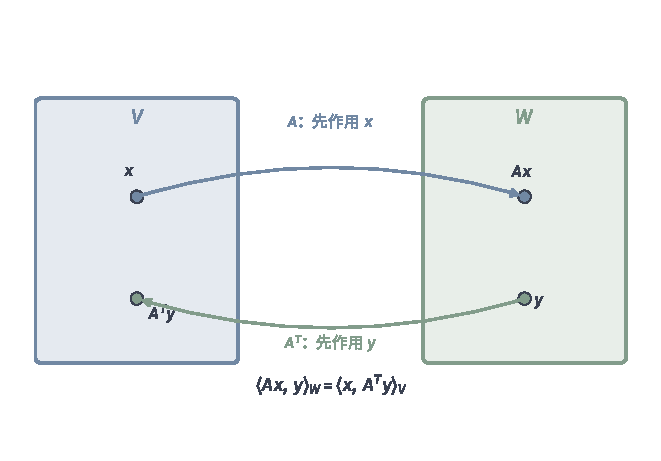
\includegraphics[width=112mm]{figures/00-shared/mathematical-preliminaries-upper/02-linear-spaces/matplotlib/ls-adjoint-action-transfer/ls-adjoint-action-transfer.pdf}
  \caption{内积伴随把输出端的配对搬回输入端。左：$T:V\to W$把$\bm x$映成$T\bm x$，与$\bm y\in W$配对；右：伴随$T^\star:W\to V$把$\bm y$映回$T^\star\bm y\in V$，使$\langle T\bm x,\bm y\rangle_W=\langle\bm x,T^\star\bm y\rangle_V$。标准欧氏内积下$T^\star$就是转置；它反转的是配对的方向，不是逆作用。箭头与空间为解析示意。}
  \label{fig:ls-adjoint-action-transfer}
\end{figure}

\paragraph{自伴、正交与正规算子}
对算子$T:V\to V$，伴随仍是$V$上的算子，可以与$T$比较。下面四类算子都由$T$与$T^\star$之间的一个等式规定。

若$T^\star=T$，称$T$为\term{自伴}（self-adjoint）算子，它在标准正交基下对应对称矩阵。若$T^\star=-T$，称$T$为\term{反自伴}（skew-adjoint）算子，它在标准正交基下对应满足$\bm A^\top=-\bm A$的反对称矩阵。反自伴算子把每个向量送到与它正交的方向：由$\langle T\bm x,\bm x\rangle=\langle\bm x,T^\star\bm x\rangle=-\langle\bm x,T\bm x\rangle$得$\langle T\bm x,\bm x\rangle=0$。例如平面上的$\left[\begin{smallmatrix}0&-1\\1&0\end{smallmatrix}\right]$把$(x_1,x_2)^\top$送到$(-x_2,x_1)^\top$，即逆时针旋转直角。

若$Q^\star Q=\operatorname{id}$，则$Q$保持内积：$\langle Q\bm x,Q\bm y\rangle=\langle\bm x,Q^\star Q\bm y\rangle=\langle\bm x,\bm y\rangle$，称为正交算子。它在标准正交基下对应第~\ref{sec:ls-orthogonal-matrices}节的正交矩阵；由方阵的单侧逆即双侧逆，$Q^{-1}=Q^\star$。

满足$TT^\star=T^\star T$的算子称为\term{正规}（normal）算子，即$T$与自己的伴随可交换。自伴、反自伴与正交算子都是正规算子：前两种情形$T^\star=\pm T$显然与$T$交换，正交算子满足$QQ^\star=Q^\star Q=\operatorname{id}$。一般算子未必正规，例如示例~\ref{ex:ls-weighted-adjoint}中的$\bm A=\left[\begin{smallmatrix}0&1\\0&0\end{smallmatrix}\right]$在欧氏内积下满足$\bm A\bm A^\top=\operatorname{diag}(1,0)\neq\operatorname{diag}(0,1)=\bm A^\top\bm A$。这些算子的谱性质在第~\ref{chap:eigen-spectral-decomposition}章讨论，这里只给出定义。

\paragraph{复空间中的泛函表示与伴随}
复空间沿用前面“第一变量共轭线性、第二变量线性”的约定。这时线性泛函应写成$\varphi(\bm x)=\langle\bm v,\bm x\rangle$，让$\bm x$处于线性的变量位置。若$\bm q_1,\ldots,\bm q_d$是标准正交基，则$\bm v=\sum_j\overline{\varphi(\bm q_j)}\bm q_j$；代入各基向量即可核对读数。表示向量随泛函作共轭线性变化，这与实空间中的线性对应不同。

例如在$\mathbb C$的标准内积$\langle v,z\rangle=\overline v z$下，泛函$\varphi(z)=(1+\mathrm i)z$对应$v=1-\mathrm i$，因为$\overline v z=(1+\mathrm i)z$。若交换两个变量的位置，得到的表达式关于$z$共轭线性，不再是线性泛函。所以共轭来自内积约定，不能从实数公式中直接删去。

两个复内积空间之间的伴随仍由$\langle T\bm x,\bm y\rangle_W=\langle\bm x,T^\star\bm y\rangle_V$定义。在标准正交基下，若$T$的矩阵为$\bm A$，伴随的矩阵就是$\bm A^*$；若两端基的Gram矩阵为$\bm M_V,\bm M_W$，则为$\bm M_V^{-1}\bm A^*\bm M_W$。这与代数对偶映射的矩阵$\bm A^\top$不同：后者只复合线性泛函，不涉及内积和共轭。复空间中，自伴矩阵满足$\bm A=\bm A^*$；保持内积的方阵满足$\bm A^*\bm A=\bm I$，称为酉矩阵。

\section{本章小结}
\label{sec:ls-dual-spaces-summary}

本章回答了章首的三个问题：线性读取组成对偶空间，读取经对偶映射在两端之间传递，读取的大小由对偶范数度量。

对偶空间由线性泛函组成，维数与原空间相同；对偶基就是坐标读取，用对偶基表示一个读取时不必解方程。对偶映射把输出端的读取传回输入端，在对偶基下记录为转置，由此又得到行秩等于列秩。这些结论只用线性运算，与范数和内积无关。

有了范数，读取就有了大小。对偶范数是读取在单位球上的最大绝对值，也就是误差受限时读取的最大变化；$\ell_p$范数的对偶范数是$\ell_q$范数，$1/p+1/q=1$，最坏方向由Hölder不等式的取等条件给出。讨论“输入误差最多引起多大输出误差”时，必须先说明误差用哪种范数度量。

有了内积，读取又可以写成向量。Riesz表示定理说明，有限维内积空间上的每个线性泛函都是与唯一一个向量的内积，内积诱导范数下对偶范数就是这个向量的长度。把对偶映射两端的读取都换成向量，就得到伴随：在标准正交基下伴随就是转置，在一般基下还要计入两端的Gram矩阵。自伴、正交与正规算子都由伴随定义，第~\ref{chap:eigen-spectral-decomposition}章的谱定理将在这类算子上展开。

